%!mode::"TeX:UTF-8"  因为WinEdt自身识别文档编码的能力不强所要求的,相当于告诉它这是UTF-8编码

%导言部分,定义文档的类型,所使用的宏包等信息,全局的设定,定义文档的通用属性

%导言部分,声明文档的类型
\documentclass{article}

%双栏表示
%\documentclass[twocolum]{article}

%页面布局
\usepackage[top = 2.54cm, bottom=2.54cm, left=3.18cm, right=3.18cm]{geometry}
%导言部分,可以加载的宏包
\usepackage{amsmath}
\usepackage{amssymb}
%\usepackage{xltxtra}  该宏在pdflatex中会报错
\usepackage{mflogo,texnames}
\usepackage{amsthm}
\usepackage{graphicx}

%导言部分,配置宏包或定义命令以供全局使用
\newtheorem{definition}{Definition}            % 前面自动加上{}中内容,显示编号,只有一个数字编号
\newtheorem*{thmwn}{Thm}                       % 前面自动加上{}中内容,不显示编号
\newtheorem{theorem}{Theorem!!!}[section]      % 后面的方括号表示该定理从属于方括号里面的内容,所以从属于section,编号从该section部分开始
\newtheorem{lemma}[theorem]{Lemma}             % lemma环境与theorem使用同一套编号
\newtheorem{proposition}{Proposition}[section]
\newtheorem{corollary}{Corollary}[theorem]     % 后面的方括号表示该定理从属于方括号里面的内容,从属于theorem,编号从theorem开始,自然从后面多一级
\newtheorem{example}{Example}

%导言部分,可以定义标题信息
\author{WP}
\title{My first \LaTeX{} article}

%正文部分,开始
\begin{document}
    %生成标题的命令
    \maketitle

    %正文输入开始
    This is my first \LaTeX{} article!

    hello world!!

    %\XeTeX{},\XeLaTeX{},\AmSTeX{},\AmS-\LaTeX{},
    %\BibTeX{},\LuaTeX{},Con\TeX{}t,
    Con\TeX{}t,

    \METAFONT,\MF,\quad,\MP

    %如何生成标题
    \section{First Section}
    this is the first section
    \subsection{First Subsection}
    I like the first subsection
    \subsection{Second Subsection}
    I don't like the second subsection
    \subsubsection{First Subsubsection}
    \paragraph{1st paragraph}
    this is the first paragraph
    \subparagraph{1st Subparagraph}
    this is the first subparagraph
    \subparagraph{2nd subparagraph}
    this the second subparagraph

    %如何输入数学符号
    \section{Second Section}
    1+1=2, $1+1=2$, I know 1+1=2, $I\ really\ know 1+1=2$
    this is in text mode, $this is in math mode,$ $this\ is\ in\ math\ in\ mode.$

    I know that you know $1+1=2$, but I know $2-1=1$, which you don't know. Now look at it $$2-1=1$$ I do know more than you.

    $\frac{2011}{2012}, x_1,x_2,\ldots,x_n, a^2+b^2=c^2, x_1^2+x_2^2+\dots+x_n^2=r^{100}, \sqrt{x+1}, \sqrt[3]{x^2+1}$

    $$\frac{2011}{2012}, x_1,x_2,\ldots,x_n, a^2+b^2=c^2, x_1^2+x_2^2+\dots+x_n^2=r^{100}, \sqrt{x+1}, \sqrt[3]{x^2+1}$$

    $\sin x, sin x, \sinh x, \max x, \log x, \log_2 x.$

    $a \in A, A \subset B, A \cap B, A \cup B, +\infty, \forall, \exists, f'(x),f''(x).$

    $\lim_{n \to\infty} a_n = 1, \sum_{n=1}^{\infty} n = 5050, \int_{a}^{b}f(x) \mathrm{d} x = I$

    $$\lim_{n \to\infty} a_n = 1, \sum_{n=1}^{\infty} n = 5050, \int_{a}^{b}f(x) \mathrm{d} x = I$$

    $$\lim_{n \to \infty} (n + \frac{1}{n})^n = e, \int_{-\infty}^{+\infty} \frac{\sin x}{x} \mathrm{d} x = I$$

    $a \times b, c \div d, a < b, b = c, c \neq d, d > e, e \geq f, f \leq g, g \geqslant h, h \leqslant i$

    $ \alpha,\beta,\gamma,\delta, \epsilon \varepsilon, \xi, \pi,\rho, \sigma, \eta, \theta, \phi, \varphi, \omega$
    $\Gamma, \Delta, \Sigma, \Phi$

    $|A|, \|A\|, \vec{a}, \overrightarrow{AB}, \tilde{x}, \widetilde{xyz}, \mathrm{sin}, \mathbb{RCZQ}, \mathbf{ABCD}$
    %web test

    % 分段函数等输入
    \begin{equation} %该输入构成一个公式环境,不需要添加美元符号,默认行间公式,自带编号
        \left(
        \begin{array}{ccc}
          a_{11} & a_{12} & a_{13} \\
          a_{21} & a_{22} & a_{23} \\
          a_{31} & a_{32} & a_{33}
        \end{array}
        \right)
    \end{equation}

    \begin{equation}
    \lim_{n \to \infty} \left( 1 + \frac{1}{n} \right)^n = e
    \end{equation}

    \begin{equation}
        \left\{
        \begin{array}{c||c|c}
          a_{11} & a_{12} & \\
          \hline
          a_{21} &  & a_{23} \\
           & a_{32} & a_{33}
        \end{array}
        \right)
    \end{equation}

    \begin{equation}
      \chi_A(x)=
      \left \{
      \begin{array}{ll}
        1, & x \in A \\
        0, & x \not\in A
      \end{array}
      \right. % 后面必须有那个点才行
      \label{myquation}
    \end{equation}


    \section{Third Section}

    %如何输入数学定理及证明
    \section{section using amsthm}
    \begin{definition}
      Definition is a environment for typing definition in \LaTeX{}.
    \end{definition}

    \begin{definition}[Theorem]
      A sentence is called a Theorem if and only if it satisfies \dots.
    \end{definition}

    \begin{thmwn}
      this is a theorem without any numbers.
    \end{thmwn}

    \begin{lemma}
      this is a lemma.
    \end{lemma}

    \begin{theorem}
      this is the first theorem with automatic number.
    \end{theorem}

    \begin{proposition}
      this is a proposition.
    \end{proposition}

    \begin{proof}
      this is a brief proof.
    \end{proof}

    \begin{theorem}[second one]         %%加入一个注释,编译后显示在定理后面
      this is the second theorem with automatic numbers.
    \end{theorem}

    \begin{corollary}
      this is a corollary.
    \end{corollary}

    \begin{proof}[My own proof]         %%加入一个注释,但是会替换掉Proof.
      this is my own proof for the corollary.
    \end{proof}

    \begin{corollary}
      this is also a corollary.
    \end{corollary}


  %如何输入图形
  
  
  \section{Section Inserting Figure}
  \begin{figure}[ht]
    \centering   %居中
    %方括号里为参数,控制图形尺寸,旋转等,其中textwidth为文章的文本宽度,angle为逆时针旋转角度。花括号是图像文件的名字,不需要扩展名
    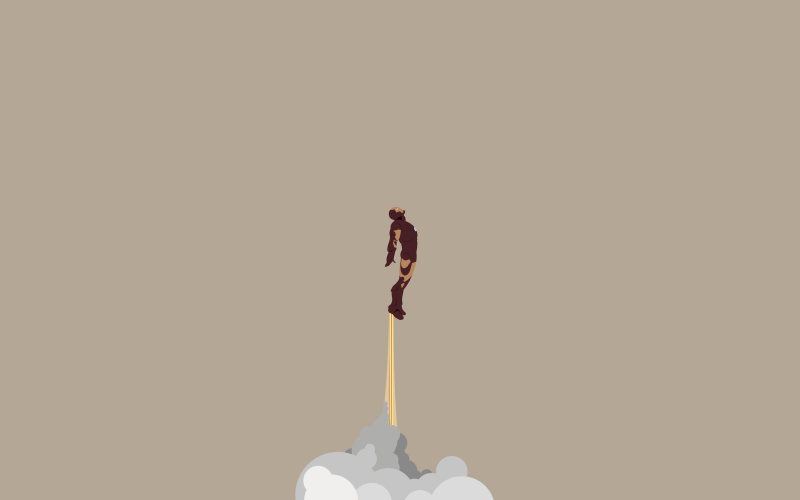
\includegraphics[width=1\textwidth, angle = 0]{3418998-simple-wallpapers}
    \caption{Elon Musk}
  \end{figure}

  %如何输入表格
  \section{Section Inserting Table}
  \begin{tabular}{l|l}
    %\hline
    % after \\: \hline or \cline{col1-col2} \cline{col3-col4} ...
    Name & Score \\
    \hline
    You & 100 \\
    Me & 59 \\
  \end{tabular}

  %\begin{table}
%    \centering
%    \begin{tabular}{|l|l|}
%      \hline
%      % after \\: \hline or \cline{col1-col2} \cline{col3-col4} ...
%      Name & Score \\
%      \hline
%      You & 100 \\
%      Me & 59 \\
%      \hline
%    \end{tabular}
%    \caption{Scores}
%    \label{myTable}
%  \end{table}

  %交叉引用
  \section{Section Cross-reference}
  equitation (\ref{myquation}) is my favorite.


%  \begin{thebibliography}{9}
%    \bibliographystyle{plain}
%    \nocite{*}\bibliography{reference}
%
%  \end{thebibliography}



\end{document}


